\section{Wave Motion}
\subsection{Progressive Waves}
\begin{defn}{Progressive wave}{}
Wave in which energy is carried from one point to another \emph{by means of vibrations or oscillations} within the waves, without transporting matter.
\end{defn}

\subsubsection{Key Terms}
\begin{defn}{Displacement $y$}{}
Distance in a specific direction of a point on the wave from its equilibrium position.
\end{defn}

\begin{defn}{Amplitude $A$}{}
Maximum displacement of any point on the wave from its equilibrium position. 
\end{defn}

\begin{defn}{Period $T$}{}
Time taken for one complete oscillation of a point in the wave.

(Time taken for wave to travel a distance of one wavelength)
\end{defn}

\begin{defn}{Frequency $f$}{}
Number of oscillations per unit time of a point on the wave.
\end{defn}

\begin{defn}{Wavelength $\lambda$}{}
Minimum distance between any two points of the wave with the \emph{same phase} at the \emph{same instant}.
\end{defn}

\begin{defn}{Wave speed $v$}{}
Speed with which energy is transmitted by wave.
\begin{equation}
v=f\lambda
\end{equation}
\end{defn}

\begin{remark}
For EM waves, $v=3\times10^8$ \unit{m.s^{-1}} in vacuum; for sound waves, $v=330$ \unit{m.s^{-1}} in air.
\end{remark}

\begin{defn}{Wavefront}{}
An imaginary line or surface joining points that are in phase.
\end{defn}

\subsubsection{Transverse and Longitudinal Waves}
\begin{defn}{Transverse wave}{}
Direction of vibration of the wave particles is \underline{perpendicular} to \emph{direction of transfer of energy} of the wave.
\end{defn}

\begin{defn}{Longitudinal wave}{}
Direction of vibration of the wave particles is \underline{parallel} to the \emph{direction of transfer of energy} of the wave.
\end{defn}

\textbf{Mechanical wave}: wave that requires a medium for propagation.
E.g.: sound waves, Water waves

\textbf{Electromagnetic wave}: wave consisting of oscillating electric and magnetic fields that are perpendicular to each other and to the direction of transfer of energy of wave. It does not require medium for transmission. It can travel through a vacuum at spedd of light.

\subsubsection{Graphical Representations}
\begin{itemize}
\item \textbf{Displacement-distance graph}

Displacement of particles at a particular instant in time.

Determine wavelength, amplitude

\item \textbf{Displacement-time graph}

Displacement of a single particle varies with time.

Determine period, amplitude

\item \textbf{Pressure-distance graph} (longitudinal waves)
\end{itemize}

\subsubsection{Phase and Phase Difference}
\textbf{Phase}: angle which indicates fraction of a cycle completed by particle / wave.

\textbf{Phase difference} $\Delta\phi$: angle which indicates how much one wave / particle is \emph{out of step} with another.
\begin{itemize}
\item \textbf{In phase}: in step with one another ($\Delta\phi=0$)
\item \textbf{Out of phase}: not in step with one another ($\Delta\phi\neq0$)
\item \textbf{Anti-phase}: out of phase by half cycle ($\Delta\phi=\pi$)
\end{itemize}

For displacement-distance graph,
\begin{equation}
\Delta\phi = \frac{\Delta x}{\lambda} \times 2\pi
\end{equation}

For displacement-time graph,
\begin{equation}
\Delta\phi = \frac{\Delta t}{T} \times 2\pi
\end{equation}

\subsubsection{Energy, Intensity}
From SHM, energy associated with oscillation is proportional to square of amplitude:
\[ E = \frac{1}{2}m\omega^2{x_0}^2 = \frac{1}{2}m(2\pi f)^2{x_0}^2 \implies \boxed{E\propto f^2A^2} \]

\begin{defn}{Intensity $I$}{}
Rate of energy transmitted per unit area perpendicular to direction of wave velocity.
\begin{equation}
I = \frac{P}{\text{Area}}
\end{equation}
\end{defn}

As a wave spreads out, its amplitude decreases. This suggests that intensity $I$ of a wave is related to amplitude $A$. At constant $f$,
\[ I\propto E \text{ and } E\propto A^2 \implies \boxed{I\propto A^2} \]

Sources of transmission
\begin{itemize}
\item Three-dimensional transmission: point source emits energy radially outwards onto spherical surface (surface area of $4\pi r^2$)
\[ I\propto\frac{1}{r^2} \]
\item Two-dimensional transmission: point source emits energy radially outwards onto cylindrical surface (surface area of $2\pi rh$)
\[ I\propto\frac{1}{r} \]
\end{itemize}
\pagebreak

\subsection{Polarisation}
\begin{defn}{Polarisation}{}
Oscillations of wave are \emph{confined to only one direction}, in the plane normal to the direction of transfer of energy of wave.
\end{defn}

\begin{remark}
Polarisation is associated only with \emph{transverse waves}. Longitudinal waves (e.g. sound waves) cannot be polarised, as they do not have oscillations in the plane normal to direction of transfer of energy of wave.
\end{remark}

\textbf{Polariser}: optical filter that allows waves of specific polarisation pass through, while blocking waves of other polarisation.

\begin{figure}[H]
    \centering
    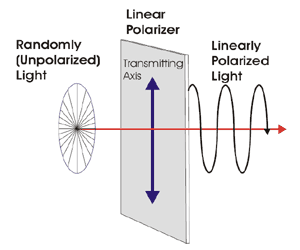
\includegraphics[width=8cm]{images/polarisation.png}
\end{figure}

\subsubsection{One Polariser}
When an unpolarised wave is incident on a polariser, its intensity is halved\footnote{because incident unpolarised wave is a random mixture of all states of polarisation, so vertical and horizontal components are, on average, equal.}, amplitude unchanged.
\begin{equation}
I=\frac{1}{2}I_0
\end{equation}

\subsubsection{Two Polarisers}
Analyser only allows \emph{component} of oscillation \emph{parallel} to transmission axis to pass through.

\begin{figure}[H]
    \centering
    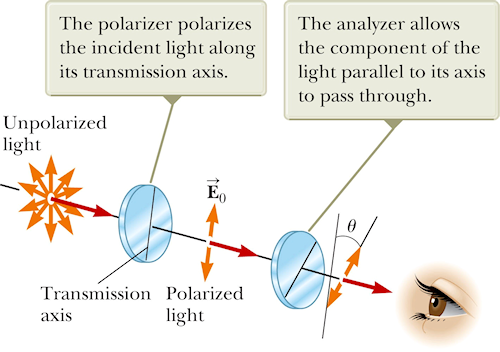
\includegraphics[width=10cm]{images/polariser_two.png}
\end{figure}

Let $I_0$ denote intensity of linearly polarised light, $I$ denote intensity after passing through analyser, $\theta$ denotes angle between direction of polarisation of incident wave and the polarising axis. Then
\begin{equation*}\tag{1}
I_0 \propto {A_0}^2
\end{equation*}
Component of $A_0$ parallel to transmission axis of analyser is $A=A_0\cos\theta$. Hence $I \propto (A_0\cos\theta)^2$, or
\begin{equation*}\tag{2}
I \propto {A_0}^2\cos^2\theta
\end{equation*}

Dividing (2) by (1) and rearranging gives \textbf{Malus' Law}:
\begin{equation}
I = I_0\cos^2\theta
\end{equation}

\begin{remark}
$I$ is maximum when transmission axes of polariser and analyser are aligned, i.e. $\theta=0\degree$; $I$ is minimum when transmission axes are perpendicular to each other, i.e. $\theta=90\degree$.
\end{remark}
\pagebreak

\subsection{Cathode Ray Oscilloscope (c.r.o.)}

\begin{figure}[H]
    \centering
    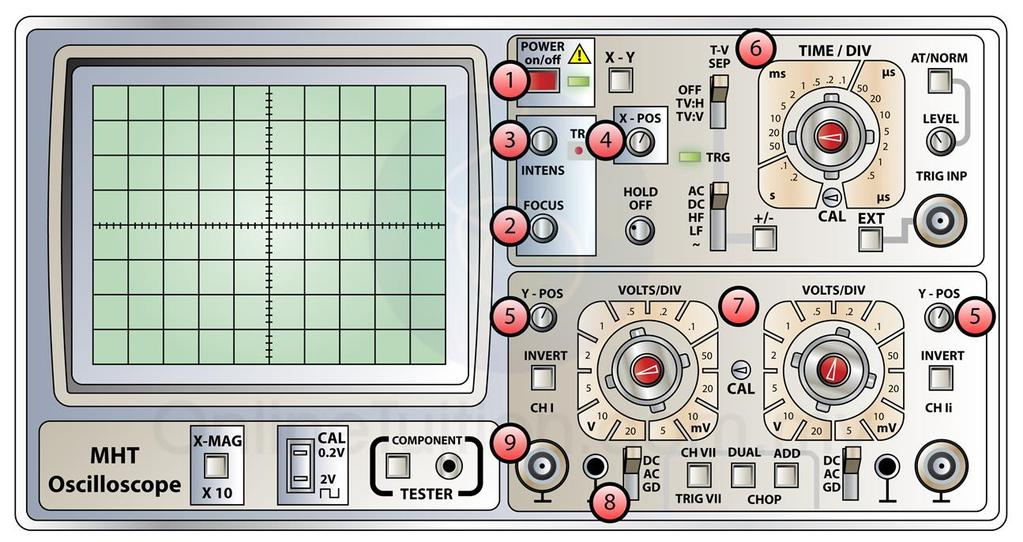
\includegraphics[width=10cm]{images/cro.jpg}
\end{figure}

Determine frequency of sound wave
\begin{enumerate}
\item Signal fed through microphone into c.r.o.
\item Turn on time-base of c.r.o., trace on screen displays displacement against time.
\item Adjust time-base until stationary trace obtained.
\item Find period $T$, calculate frequency $f$ using $f=\dfrac{1}{T}$.
\end{enumerate}

Determine wavelength of sound wave (using stationary waves)
\begin{enumerate}
\item Loudspeaker delivers sound via signal generator. Incident wave is directed towards and is reflected at reflecting board.
\item Superposition of incident wave and reflected wave produces stationary wave in the space between loudspeaker and reflecting board.
\item Connect microphone to c.r.o. (time-base switched off\footnote{so that the spot does not move across the screen. The spot moves up and down the screen, and the height of the vertical trace gives a measure of the amplitude of the sound}). Move it along the line between loudspeaker and reflecting board.
\item When microphone is at positions of minimum amplitude (nodes), signal displayed is minimum; at positions of maximum amplitude (antinodes), signal displayed is maximum.
\item Measure distance across several nodes / antinodes, calculate average distance $d$ between two adjacent nodes / antinodes.
\item Separation of two adjacent nodes is equal to half a wavelength: $d=\dfrac{1}{2}\lambda$.
\end{enumerate}

\begin{figure}[H]
    \centering
    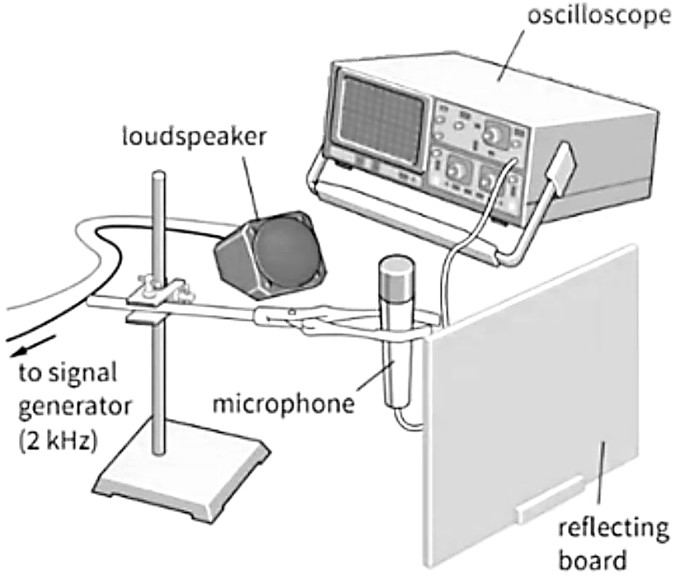
\includegraphics[width=10cm]{images/cro_wavelength.jpg}
\end{figure}

\begin{exercise}{}{}
Suggest why it is easier to determine accurately the position of a node rather than an antinode.
\end{exercise}
\begin{proof}[Answer]
The amplitude of oscillation at a node is zero. Hence it is easier to see the spot on the screen lie right on the horizontal line.
\end{proof}

\begin{exercise}{}{}
Explain why it is better to measure the distance across several nodes.
\end{exercise}
\begin{proof}[Answer]
Measuring a longer distance produces a smaller relative error of measurement.
\end{proof}

\pagebreak

\subsection*{Problems}
% https://www.topperlearning.com/answer/two-polarizers-are-placed-at-crossed-position-ie-having-an-angle-of-90-between-them-a-third-polarizer-making-an-angle-with-the-first-one-is-placed-bet/jbjws733
\pagebreak